\section{Rozwiązanie problemu} 

\begin{frame}
    \frametitle{Integracja modeli symulacyjnych}
    \begin{figure}
        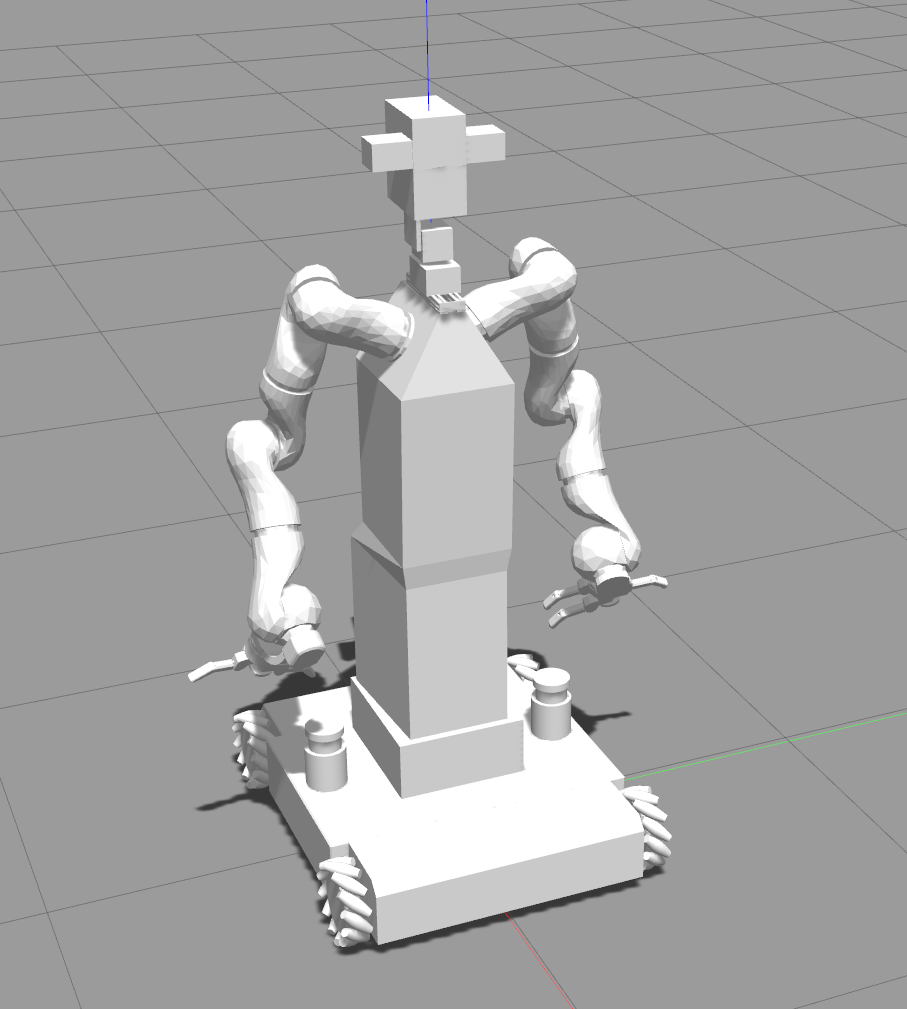
\includegraphics[scale=0.20]{./images/omnivelmobil-final-cropped.png}
        \caption{Zintegrowany robot Velma w symulatorze Gazebo}
    \end{figure}
\end{frame}

\begin{frame}
    \frametitle{Ogólna struktura projektowanego systemu} 
    %% tutaj wrzucić sysmla z ogólną budową systemu - podział na część symulacyjną i sterującą
\end{frame}

\begin{frame}
    \frametitle{Struktura symulatora robota Velma} 
    %% opis części symulacyjnej - podział na modele, silnik i wtyczki
\end{frame}

\begin{frame}
    \frametitle{Zasada działania kontrolera bazy mobilnej} 
    %% opis zmian które zaszły w kontrolerze bazy mobilnej po zmianie silnika fizyki
\end{frame}

\begin{frame}
    \frametitle{Struktura systemu sterowania} 
    %% opis systemu sterującego - opis sterowania częścią manipulacyjną i bazą mobilną
\end{frame}




